\documentclass[12pt]{article}
\usepackage{amsmath}
\usepackage{amssymb}
\usepackage[letterpaper,top=1.35in,bottom=0.75in,left=0.75in,right=0.75in,centering]{geometry}
\usepackage{fancyhdr}
\usepackage{enumerate}
\usepackage{lastpage}
\usepackage{multicol}
\usepackage{graphicx}
\usepackage{vwcol}
\reversemarginpar

\pagestyle{fancy}
\cfoot{Page \thepage \ of \pageref{LastPage}}\rfoot{{\bf Total Points: 18}}
\lhead{\hspace*{2.2in}\underline{MATH 1560: Test 3}}

\newcommand{\points}[1]{\marginpar{\hspace{24pt}[#1]}}
\newcommand{\skipline}{\vspace{12pt}}
\renewcommand{\headrulewidth}{0in}
\headheight 20pt

\newcommand{\di}{\displaystyle}
\newcommand{\abs}[1]{\lvert #1\rvert}
\newcommand{\R}{\mathbb{R}}
\newcommand{\C}{\mathbb{C}}
\renewcommand{\P}{\mathcal{P}}
\DeclareMathOperator{\nul}{null}
\DeclareMathOperator{\range}{range}
\DeclareMathOperator{\spn}{span}
\newcommand{\len}[1]{\lVert #1\rVert}
\newcommand{\Q}{\mathbb{Q}}
\newcommand{\N}{\mathbb{N}}
\renewcommand{\L}{\mathcal{L}}
\newcommand{\dotp}{\boldsymbol{\cdot}}
\newenvironment{amatrix}[1]{%
  \left[\begin{array}{@{}*{#1}{c}|c@{}}
}{%
  \end{array}\right]
}
\newcommand{\bam}{\begin{amatrix}}
\newcommand{\eam}{\end{amatrix}}
\newcommand{\bbm}{\begin{bmatrix}}
\newcommand{\ebm}{\end{bmatrix}}

\begin{document}


\author{Instructor: Sean Fitzpatrick}
\thispagestyle{plain}
\begin{center}
\emph{University of Lethbridge}\\
Department of Mathematics and Computer Science\\
17 October, 2017\\
{\bf MATH 1560 - Test \#3 -- Individual Stage}\\
Examiner: Sean Fitzpatrick
\end{center}
%\skipline \skipline \skipline \noindent \skipline
%Last Name:\underline{\hspace{350pt}}\\
%\skipline
%First Name:\underline{\hspace{348pt}}\\
%\skipline
%Student Number:\underline{\hspace{322pt}}\\
%\skipline



\vspace{0.1in}

\vspace*{\fill}

\begin{quote}
Print your name and student number clearly in the space above. You may remove this cover page, and use the back for scrap paper. If you want any work on the back of this page to be graded, you must clearly indicate this on the page containing the corresponding question.

\medskip

Answer the questions in the space provided. Show all work and necessary justification. Partial credit may be awarded for partially correct work.
 
\medskip

No outside aids are permitted, with the exception of a basic calculator. 
\end{quote}



\newpage

This page left intentionally blank. You may use this page for rough work.
\newpage

 \begin{enumerate}
 \item  Calculate the derivative of $f(x) = \arctan(x^2)$. \points{2}
 
 \vspace{4cm}
 
 \item Calculate the derivative of $f(x) = \sqrt{\dfrac{x^3e^x}{x^6+2x^2}}$. \points{4}\\
 Suggestion: use logarithmic differentiation.
 
 \vspace{6cm}
 
 \item Use implicit differentiation to compute $\dfrac{dy}{dx}$ (in other words, $y'$) if \points{4}
 \[
 x^4+x^2y^2=3y.
 \]
 
 \newpage
 
 \item Determine the absolute (global) maximum and minimum values of $f(x) = x^2+\dfrac{1}{x}$ on the interval $[\frac{1}{10},2]$. \points{4}

  
  \vspace{10cm}
  
 \item This question refers to the graph of a function $f$ shown below on the right. For each value requested below, either enter the value, or DNE, if the value is undefined. You do not have to explain your answer.\points{4}
 \begin{multicols}{2}
 \begin{enumerate}
 \item What is the absolute maximum of $f$?\\
 (Give both $x$ and $y$ coordinates)
 
 \vspace{1cm}
 
 \item What is the absolute minimum of $f$?\\
  (Give both $x$ and $y$ coordinates)

\vspace{1cm}

\item At what $x$ coordinate(s) is $f'(x)=0$?
 \end{enumerate}
 \begin{center}
 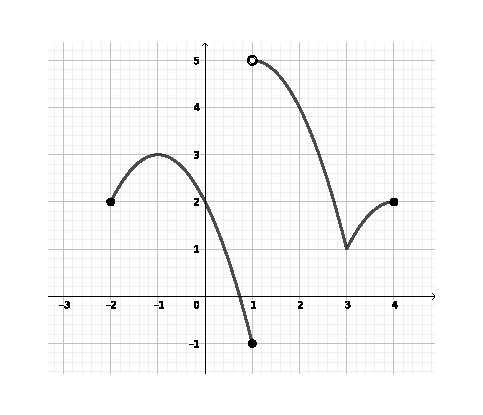
\includegraphics[width=0.9\columnwidth]{TT3_fig1}
 \end{center}
 \end{multicols}
 
 
 
\begin{enumerate}
\addtocounter{enumii}{3}

\vspace{1cm}

\item At what $x$ coordinate(s) does $f'(x)$ not exist?
\end{enumerate}
\end{enumerate}
\end{document}